\documentclass[letterpaper,11pt]{article}

\usepackage{amsmath} 
\usepackage{amsthm} 
\usepackage{amsfonts} %required for \mathbb
\usepackage{listings}
\usepackage{color}
\usepackage{listings}
\usepackage{graphicx}
\usepackage{setspace}
\usepackage{float}
\usepackage{hyperref}
\usepackage{courier}

\definecolor{lightgray}{gray}{0.95}
\hypersetup{
hidelinks}

\lstset{breaklines=true,
    language=Lisp,
    basicstyle=\footnotesize\ttfamily, 
    backgroundcolor=\color{lightgray},
}



\begin{document}
\title{MLang: Musical Language}
\author{Aditya Mukerjee, Nikhil Sarda, Nistha Agarwal, Sushmita Swaminathan}
\maketitle

\section{Introduction}

Aesthetics are by nature subjective and non-deterministic; as such, a programming language cannot fix this problem. But aesthetics are often determined by adherence to well-defined artistic conventions. Just as a simple Venician sonnet must have a fixed meter and rhyming scheme, musical compositions such as fugues, canons, and concertos must obey a well-defined structure specific to that musical form. When composing classical music, a deep understanding of music theory and strong grasp of music notation and grammar are required simply to create a piece compliant with the accepted contemporary musical structure - and that is all before beginning any part of the creative, artistic process. 

However, while the underlying theory is vast, these conventions are extremely well-defined. As a result, most of this process can be facilitated by use of a piece of software specific enough to be tailored to the individual piece of music at hand, yet powerful enough to allow the composer to break free of conventions when necessary, or even to redefine or extend the set of rules. Traditionally, this software is implemented as a graphical frontend to standard music notation. The creators of MLang believe that undermines the power of music. Music is itself a language, and a composition is simply an application of the language, just as a program is an application of a programming language.

The language we have described is simply the language of music - simple and minimal, yet powerful. The same is true of homoiconic functional programming languages, which made the selection of a programming paradigm MLang rather clear. Homoiconic functional languages are simple, yet highly powerful, and they derive this power through their modularity.

MLang is a language that helps its users compose music by writing and compiling programs. It is a homoiconic functional language that is simple,
yet highly powerful, and modular. Many of MLang's features are similar to a functional programming language like LISP. 
Thus, familiarity with functional programming languages and a basic knowledge of music is preferred but not required.


\subsection{Modularity}
Music itself is highly modular. Not only is it common for sections of music to be repeated exactly within a given piece of music, but it is often expected that variations on these sections be repeated within the same composition. Subsequently, these sections may included in later compositions by other authors. All music is thus, in some sense, derivative - it is the nature of the art form.  

MLang exposes this modularity, intrinsic in music, and turns it from a barrier to entry into a tool for the beginning composer (and instructors of music composition). Like standard music composition software, MLang allows composers to create music from scratch, by defining notes individually.  Thus, a user familiar with traditional music notation would have little trouble adjusting to MLang. Most music composition software provides this feature and little else. MLang, however, takes this a step further, by allowing the composer to extract arbitrary elements from that music and bundle these elements together into a module.

\subsection{Metaprogramming}
MLang allows the user to incorporate other pieces of MLang code - which are playable music files - into their own code as modules. A module is not limited to being just a complete musical phrase, such as a measure, a note, or an entire movement. It may be an attribute of the music, such as the key, time signature, or timbre - these attributes are not necessarily observed (ie, heard) in just a single section of the composition, but rather, they are woven into the composition as a whole. 


\subsection{Homoiconicity}
A language is said to be homoiconic if a representation of programs written in it are also a data structure in a primitive type of the language itself. In MLang, the only primitive is a series (list, these lists may be of length one) of musical tones (a note), or a function. However, because functions are themselves stored internally as series of certain musical tones, everything in MLang, including the code itself, is a representation of a series (list) of notes. Modules, the higher-level data structures, are themselves recursively composed of other modules or of primitives (notes). So the code itself has a recursive representation as a primitive datatype. For MLang, the elementary datatype is an m-expression. We define an M-expression inductively as 
1. a musical note, or
2. an expression of the form (x . y) where x and y are m-expressions.
Note the analogous relationship between an m-expression and an s-expression.

\subsection{Functional}
MLang is stateless and free of side effects. It treats computation (generation of music) as simple evaluation of m-expressions and avoids state and mutable data. MLang is heavily influenced by the syntax and semantics of Lisp and its variants, though the interpreter itself is written in OCaml. MLang is strongly typed and dynamic.


\section{Language Tutorial}

\subsection{Conventions}

In this tutorial > refers to the command line prompt and {> refers to the
output of the MLang command.

\subsection{Data Types}
The basic data type in MLang is an MNote. An MNote is a list of length 1
and can be thought of as a function with no arguments.
An MNote can be represented as 

\lstset{breaklines=true,language=Lisp}
\begin{lstlisting}
(%rest %A %octave), 
\end{lstlisting}

where A refers to any musical note.
\lstset{breaklines=true,language=Lisp}
\begin{lstlisting}
> (label A (8 A 3))
\end{lstlisting}

In order to play the above, we can write

\lstset{breaklines=true,language=Lisp}
\begin{lstlisting}
> (label A (8 A 3))
> (read-file stdlib.mlang)
> (midge-export test.mg ((100 4 4) ((piano_grand_ac 80 1 (A)))))
> (label A (8 A 3))
\end{lstlisting}
The midge-export function takes two arguments, the filename and the song m-expression. A song is represented as a head and a body. The head contains
information such as tempo and time signature. The body consists of several channels. A channel has information such as the instrument, volume, repetitions and the notes themselves.

In the above example, the head is (100 4 4) which represents a tempo of 100 bpm and a time signature of 4/4.
There is a single channel and a single note. The instrument of choice is grand piano, volume is 80 and the A note on the 3rd octave is played once
with a 1/8 rest.

Go back to the terminal and you will see a test.mg file has been created. In order to play it type

\lstset{breaklines=true,language=bash}
\begin{lstlisting}
# midge test.mg
# banshee test.mid

\end{lstlisting}

\subsection{Input and Output}
The input for MLang would consists of codes written at the command line or as part of a fille with the .mlang extension.
The code is a series of mexpressions that represent notes, functions and other metadata.
On compilations, the program would produce a file with the .mg extension which can be postprocessed with Midge in order to produce a .mid file.

\subsection{MLang Expressions}

The common form of an MLang expression is a function application given by the syntax

\lstset{breaklines=true,language=Lisp}
\begin{lstlisting}
(function arg1 arg2 ...)
\end{lstlisting}
where the arguments can be MNotes or other functions.

MLang expressions are case insensitive: (A 100) and (a 100) mean the same

\subsection{Functions as values}

Since MLang is a homoiconic language, functions can be treated as data that can be passed around.
In MLang, all functions are evaluated to notes. Thus every function eventually is evaluated to a string of notes that forms the midi.

\lstset{breaklines=true,language=Lisp}
\begin{lstlisting}
> (MAPCAR TRANSPOSE ((4 A 3) (4 B 3) (4 C 3)))
\end{lstlisting}

where the arguments can be MNotes or other functions.
For instance, TRANSPOSE is a function that is passed as an argument to another function, in this case MAPCAR. MAPCAR applies TRANSPOSE to each
of the MNotes in the third m-expression

Another example
\lstset{breaklines=true,language=Lisp}
\begin{lstlisting}
> (read-file stdlib.mlang)
> (LABEL BASSPHRASE
  	 (CONCAT (REPEAT4 (3 B 16)) (REPEAT4 (3 A 16)) (REPEAT4 (3 G 16)) (REPEAT4 (3 A 16))))
\end{lstlisting}

Here REPEAT4 is a lambda function defined in stdlib.mlang. It takes a parameter and returns an mexpression containing it 4 times. CONCAT takes
all of these m-expressions and concatenates them.


\subsection{Writing Your First MLang Program}
Here is an example .mlang program that plays the first few notes of Happy Birthday

\lstset{breaklines=true,language=Lisp}
\begin{lstlisting}
((read-file stdlib.mlang)
	(label head
	       (42 4 4))
	(label phrase1
	       ((3 g 4) (3 g 4) (3 a 4) (3 g 8)))
	(label channel1
	       (bass_ac 96 1 phrase1))
	(MIDGE-EXPORT
		happy.mg (head (channel1))))
\end{lstlisting}

The first statement is used to load the standard library.

The label keyword is used to bind a string with an m-expression. Here we have bound head with the mexpression (42 4 4).
We have then defined the first phrase which consists of 4 notes. The label channel1 is made up of phrase1. An m-expression is then created
which is fed into midge-export.

In order to play this song from the commandline type
\lstset{breaklines=true,language=bash}
\begin{lstlisting}
# ./mlang < happy.mlang && midge happy.mg && banshee happy.mid
\end{lstlisting}

MLang is portable in the sense that it does not depend upon the machine’s hardware for its execution.

\subsection{Working with higher-order functions}


Here we show how one can use higher-order functions in order to write compact mlang programs.

\lstset{breaklines=true,language=Lisp}
\begin{lstlisting}
> (LABEL REVERSECHANNEL
       (LAMBDA (X)
                      ((CAR X) (NTH 1 X) (NTH 2 X) (REVERSE (NTH 3 X)))))

\end{lstlisting}
This is a function that reverses the fourth mexpression in a given mexpression. For instance

\lstset{breaklines=true,language=Lisp}
\begin{lstlisting}
> (REVERSECHANNEL (1 2 3 (A B C)))
(1 2 3 (C B A))
> (REVERSECHANNEL (1 2 3 (A B C)))
\end{lstlisting}
Let us make use of REDUCE, our version of a left fold.

\lstset{breaklines=true,language=Lisp}
\begin{lstlisting}
> (REVERSECHANNEL (1 2 3 (A B C)))
> (LABEL GG (LAMBDA (X Y) (CONCAT X Y)))
> (REDUCE GG ((A B) (C D)) nil)
(nil A B C D)

\end{lstlisting}
REDUCE takes three parameters, a function that takes two arguments (accumulator and element) followed by an mexpression and the initial value.
It then proceeds to left fold the mexpression using the given function.

		      
\section{Language Reference Manual}


\subsection{Lexical Conventions}

 Aditya: Please fill up


\subsection{Character Set}


Mlang programs are written in ASCII character set.


\subsection{Identifiers}

In MLang, an identifier is a string that starts with a letter or an underscore, and consists
of a sequece of letters, digits, and underscores. Identifiers are case insensitive.


\subsection{Keywords}


The following keywords are reserved 


\begin{list}{}{}
\item \texttt{  QUOTE }
\item \texttt{ CAR }
\item \texttt{ CDR }
\item \texttt{  SETCAR }
\item \texttt{ SETCDR }
\item \texttt{ CONS }
\item \texttt{  EQUAL }
\item \texttt{ ATOM }
\item \texttt{ COND }
\item \texttt{  IFELSE }
\item \texttt{  LAMBDA }
\item \texttt{  LABEL }
\item \texttt{ READ-FILE }
\item \texttt{ WRITE-FILE }
\item \texttt{  LENGTH }
\item \texttt{  NTH }
\item \texttt{  LAST }
\item \texttt{  MAPCAR }
\item \texttt{  REDUCE }
\item \texttt{  INC }
\item \texttt{ DEC }
\item \texttt{  COMBINE }
\item \texttt{ REVERSE }
\item \texttt{ CONCAT }
\item \texttt{ MIDGE-EXPORT }
 \end{list}
These are simply functions whose behavior has been defined in OCaml.

\subsection{Types}


The basic type in MLang is the Mexp which is a cell. The Mexp is defined as

\lstset{breaklines=true,language=ml}
\begin{lstlisting}
type ('a, 'b) cell = { mutable car: 'a; mutable cdr: 'b }

type t = Atom of string
  | Cons of (t, t) cell
  | Func of (t -> (string, t) Hashtbl.t -> t)
  | Lambda of t * t
  | Null

\end{lstlisting}


Thus our language only provides symbol atoms (no integers, strings, etc)
and cons cells. It is dynamically scoped.


\subsection{M-expressions}


The following are valid m-expression
\lstset{breaklines=true,language=Lisp}
\begin{lstlisting}
> (1 2 3 4)

> (A B C)

> (LENGTH (1 2 3))

> (LABEL A (a l p h a))

\end{lstlisting}
\subsection{Grammar}


The grammar of Mlang is incredibly simple.
It has expressions, which are symbolic identifiers, and lists.
A list is a left parenthesis followed by some number of expressions (separated by spaces) followed by a right parenthesis.

expr:   ID | list
list:   ( seq )  
seq:       | expr seq

\subsection{Higher-order functions}

%# Sushmita/Aditya please fill up with a description. Ping me if you
are not sure.

1) CONS

2) CDR
....

n) MIDGE-EXPORT: See the next section


\subsection{Midge backend}


MIDGE-EXPORT takes 2 arguments, the name of the output file and an m-expression representing the song of the midi file. 

\lstset{breaklines=true,language=Lisp}
\begin{lstlisting}
(MIDGE-EXPORT name.mg SONG)
\end{lstlisting}
The song is an m-expression represented as:

\lstset{breaklines=true,language=Lisp}
\begin{lstlisting}
(HEAD BODY)

HEAD -> (TEMPO SIGNATURE_NUMERATOR SIGNATURE_DENOMINATOR)
\end{lstlisting}

Head consists of the song of the tempo, numerator and denominator of the time signature.

\lstset{breaklines=true,language=Lisp}
\begin{lstlisting}
BODY -> (CHANNEL1 CHANNEL2 CHANNEL3....)

\end{lstlisting}
A body is a sequence of channels.

\lstset{breaklines=true,language=Lisp}
\begin{lstlisting}
CHANNEL1 -> (INSTRUMENT VOLUME REPETITION (NOTE1 NOTE2 NOTE3...))

\end{lstlisting}
A channel is represented by its instrument, volume in the mix, the number of times it must be repeated and finally, the sequence of notes.

\lstset{breaklines=true,language=Lisp}
\begin{lstlisting}
NOTE1 -> (rest note-literal octave)

\end{lstlisting}
For instance the A note on 3rd octave played as a quarter note can be
represented as

\lstset{breaklines=true,language=Lisp}
\begin{lstlisting}
(4 A 3)
\end{lstlisting}

\section{Translator Architecture (Nikhil Sarda, System Architect)}
\subsection{Architecture}

        \begin{figure}[H]
            \centering
            \makebox[0cm]{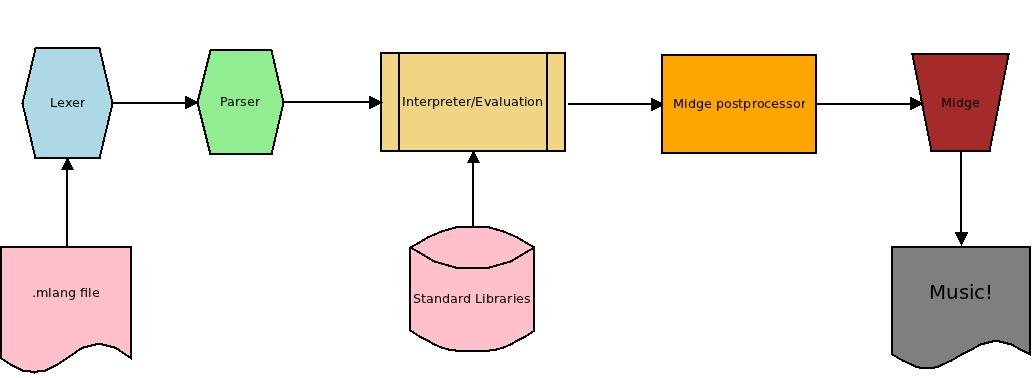
\includegraphics[scale=.2]{ArchitectureDiagram.jpg}} 
        \end{figure}
The above is a high-level overview of the architecture of the MLang compilation process. The mlang program goes through the lexer and parser that
generate an ML representation of a m-expression. This representation is then evaluated and processed into an m-expression that can be understood
by the Midge backend. If at this point definitions present in the standard library are needed, they are loaded as well.
We have defined some in built functions as well as several functions written in MLang itself. Functions written in OCaml were done so in order to
take advantage of tail-call optimization and other performance reasons. However, keeping in line with the design goal of MLang as a homoiconic
music language, NO music specific function was written in OCaml. M-expression evaluation is quite straightforward. As we walk the AST, we pattern-
match specific m-expression forms. For instance, if we encounter an atom, we check it against a hash-table that represents all the environment
variables and their respective mexpression bindings. If a binding exists, it is replaced in place of that atom and evaluated with the rest of the
m-expression treated as arguments. If not, we move on to the next m-expression. Forms such as lambdas and function calls are evaluated similarly.
The backend then generates intermediate .mg files which is then converted to MIDI. If a MIDI synthesizer is present on the system, it can be played 
with any conventional player.

\subsection{Interesting technical notes}

MLang has no side-effects. The only IO it can do is through the READ-FILE, WRITE-FILE and EXPORT-MIDGE keywords. This functionality piggy-backs on
OCaml.

Evaluation in MLang is eager.

Garbage collection in MLang piggy-backs on the OCaml run-time.

\subsection{Module Contributions}
Nikhil Sarda: Lexer, parser, most of the interpreter/evaluator, midge backend, standard library functions (translation of standard library from Lisp to pure Mlang.)
Sushmita Swaminathan: READ-FILE, WRITE-FILE function
Aditya Mukerjee: Standard library functions (pure Lisp lambda implementation), datatype fixed-point combinator, testing framework, fixes to the interpreter, repository sanitization


\section{Development and run-time environment (Nikhil Sarda)}

\subsection{Environment}


We used OCaml for all our development purposes. The compiler used was The Objective Caml toplevel, version 3.12.1 along with the Batteries Included
standard library. We used GNU Make for our build process after evaluating and rejecting OCamlBuild. Shell scripts were used as glue.
For most editing tasks, we used vim and emacs. Keeping in line with our preferences for extensible and fast editors instead of full
blown IDEs, we developed an emacs-mode for MLang as well. For version control, we used Git. This allowed us to work with multiple branches in a
completely distributed manner and allowed for easy merging when we needed to integrate the various components that different people were working on.
We used Github for source code hosting as well as for issue tracking. Email was used extensively for technical discussions.

\subsection{Build Process}
\lstset{language=bash}
\subsubsection{Makefile}
\begin{lstlisting}
OCAMLC=ocamlc
OCAMLOPT=ocamlopt
OCAMLDEP=ocamldep
INCLUDES=
OCAMLFLAGS=$(INCLUDES) -g
OCAMLOPTFLAGS=$(INCLUDES)

MAIN_OBJS=mexp.cmo midge.cmo parser.cmo lexer.cmo symtab.cmo environment.cmo builtins.cmo main.cmo

mlang: .depend $(MAIN_OBJS)
	$(OCAMLC) -o mlang $(OCAMLFLAGS) $(MAIN_OBJS)

.SUFFIXES: .ml .mli .cmo .cmi .cmx .mll .mly

.mll.ml:
	ocamllex $<
.mly.ml:
	ocamlyacc $<
.ml.cmo:
	$(OCAMLC) $(OCAMLFLAGS) -c $<

.mli.cmi:
	$(OCAMLC) $(OCAMLFLAGS) -c $<

.ml.cmx:
	$(OCAMLOPT) $(OCAMLOPTFLAGS) -c $<

testmlang: $(MLANG)
	./run_test.sh test_repl_input.txt

clean:
	rm -f mlang
	rm -f *~
	rm -f *.cm[iox]
	rm -f parser.ml parser.mli
	rm -f lexer.ml

parser.cmo : parser.cmi
parser.mli : parser.mly
parser.ml : parser.mly


.depend:
	$(OCAMLDEP) $(INCLUDES) *.mli *.ml *.mly *.mll > .depend

include .depend
\end{lstlisting}

\subsubsection{.depend}
\begin{lstlisting}
\end{lstlisting}

\subsubsection{.depend}
\lstset{language=bash}
\begin{lstlisting}
builtins.cmo: symtab.cmo mexp.cmo environment.cmo midge.cmo
builtins.cmx: symtab.cmx mexp.cmx environment.cmx midge.cmx
environment.cmo: mexp.cmo
environment.cmx: mexp.cmx
main.cmo: symtab.cmo mexp.cmo environment.cmo builtins.cmo midge.cmo
main.cmx: symtab.cmx mexp.cmx environment.cmx builtins.cmx midge.cmx
midge.cmo: mexp.cmo
midge.cmx: mexp.cmx
mexp.cmo:
mexp.cmx:
symtab.cmo: mexp.cmo
symtab.cmx: mexp.cmx
\end{lstlisting}

\subsubsection{run\_test.sh}
\lstset{language=bash}
\begin{lstlisting}

#A very basic, very hacky unit testing framework

filename=$1

repl_test()
{
    failed=0
    echo "Begin tests"
    while read p; do
        mlang_input=$(echo $p | cut -d '|' -f1)
        mlang_output=$(echo $mlang_input | ./mlang  | cut -b 1-2 --complement | head -n 1| sed 's/^ *//g' | sed 's/ *$//g')
        desired_ouput=$(echo $p | cut -d '|' -f2 | sed 's/^ *//g' | sed 's/ *$//g')
        if [ "$mlang_output" = "$desired_ouput" ]
        then
            echo ".............passed $p"
        else
            echo "!FAILED: $mlang_input produced $mlang_output instead of $desired_ouput"
            failed=`expr $failed + 1`
        fi
    done < $filename
    exit $failed
    
}

repl_test $filename

\end{lstlisting}


\subsection{Runtime Environment}
Instead of creating a separate compiler, we leveraged the REPL to act as a compiler. This was accomplished by adding a keyword MIDGE-EXPORT, which
creates the respective .mg file. We then post-process it using midge and run it with our music player of choice. For instance, if you wished to
compile a .mlang program, you would write

\lstset{language=bash}
\begin{lstlisting}
# ./mlang < my-program.mlang && midge my-program.mg && banshee my-program.mid
\end{lstlisting}
To simplify this, we created a small shell script called mlangc which does all of this automatically.

Please note that in order to run an mlang program, the user must install Midge as well as a MIDI synthesizer. Midge has a further dependency on
Perl.



\end{document}
